\documentclass[12pt, twoside,a4paper]{report}
\oddsidemargin = 10pt
\textwidth = 430pt

%\usepackage{float}
\usepackage{fullpage}	 %to make smaller margins
\usepackage{graphicx}
%\usepackage[utf8]{inputenc}
%\usepackage[T1]{fontenc}
%\usepackage{url}
\usepackage{hyperref}
\usepackage{pdfpages}
\usepackage{graphicx}
%\usepackage{caption}
\usepackage{subfig}
\usepackage{enumerate}
\usepackage{listings} %for showing program code
\usepackage{fixltx2e}

\lstset{backgroundcolor={\color{white}}, %old formatting for program listings I used in my bachelor thesis ;)
basicstyle={\bfseries\ttfamily\footnotesize},
breakatwhitespace=false,
breaklines=true,
captionpos=b,
columns=fullflexible,
commentstyle={\color[rgb]{0.133,0.545,0.133}},
escapeinside={\%*}{*)},
fontadjust=true,
frame=single,
identifierstyle={\ttfamily},
keywordstyle={\bfseries\ttfamily\color[rgb]{0,0,1}},
language=C++,
numbers=left,
numbersep=5pt,
numberstyle={\footnotesize},
showspaces=false,
showstringspaces=false,
showtabs=false,
stepnumber=1,
stringstyle={\ttfamily\color[rgb]{0.627,0.126,0.941}},
tabsize=2}

\usepackage{wrapfig}
\usepackage{lipsum}
\usepackage{float}
\usepackage{titlesec}	

\titlespacing*{\chapter}{0pt}{-10pt}{20pt}
\titleformat{\chapter}[display]{\normalfont\huge\bfseries}{\chaptertitlename\ \thechapter}{20pt}{\Huge}

\setlength{\intextsep}{0pt} %to make wrapfigures beautiful
\setlength{\oddsidemargin}{0.5cm}
\setlength{\evensidemargin}{-0.5cm}

\begin{document}

\tableofcontents
\chapter{Motivation}
Even though global illumination techniques have come a long way they still have many limitations. One of them is the often long render times they require and the difficulties of implementing and working with them efficiently. Ambient occlusion is a rather simple technique that allows indirect lighting from an envirornment to be simulated cheaply. The technique was originally developed by Hayden Landis and colleagues at Industrial light and Magic to accomodate the needs they had for production ready global illumination \cite{Landis2002}. Ambient occlusion together with envirornment mapping is therefore often used in the industry since they besides being faster also allows for easy compositing of synthetic 3D images into live video footage\cite{Landis2002}. Ambient occlusion is therefore an often used lighting technique in the movie industry.
\\ \\
We will in this report present an implementation of Ambient Occlusion into the Raytracing framework used for the course " - Rendering"

\chapter{Theory}
This section will explain the basic theory and concept behind Ambient Occlusion. Besides covering the basic concept and math behind ambient occlusion it will also be covered how texture lookup into light probe images are performed. The chapter will conclude with a discussion of the disadvantages of ambient occlusion.
\section{The Basic Concept}
Ambient Occlusion works by seeing how much of an external envirornment can be seen from each surface point on the object or scene to be rendered. The more of the external envirornment that can be seen, the more ambient lighting that point will recieve. This type of illumination is therefore often called "sky light" in production, because it simulates how a model would be lighted on an overcast day, since the light from ambient occlusion is incident on the point from all directions due to the scatering of the clouds.
\\ \\
When ambient occlusion is calculated two factors are obtained. The first is the accessibility term. This is the measure of how much of the envirornment that is accessible from the surface point. The other is the "bent normal", which is the average direction of the incident light from the envirornment. The bent normal can then be used to look up into a light probe, which is a special type of image, in order to give more realistic lighting without the added cost of a global illumination algorithm. These two concepts is illustrated on figure \ref{fig:overview} that illustrates how these two variables are calculated in a ray tracer.
\begin{figure}[h]
	\centering	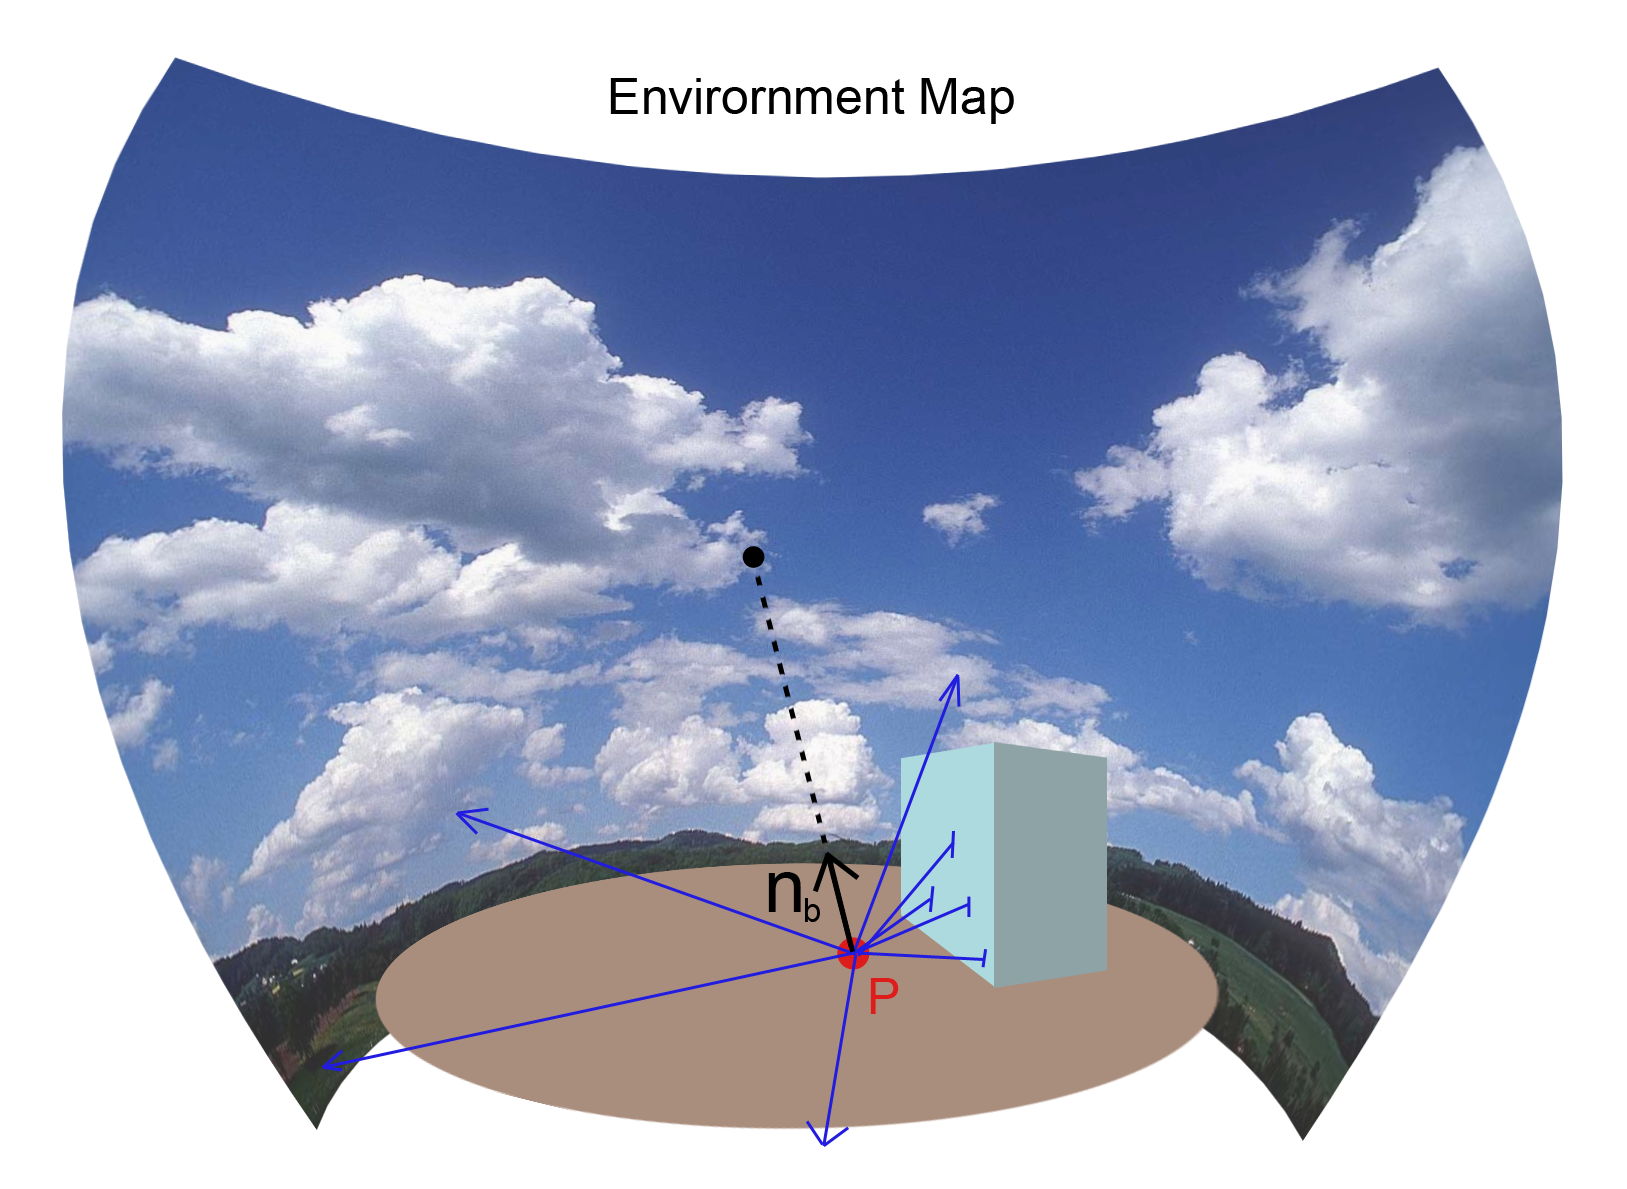
\includegraphics[width=0.6\textwidth]{Theory/overview}\caption{Overview of ambient occlusion.}\label{fig:overview}
\end{figure}
The accessibility at point P is determined by shooting rays out from the hemisphere surrounding the surface around P. The number of rays that does not hit other objects determines the accesibility. The average of the unoccluded rays is the bent normal that can be used to make a lookup into an envirornment map such as a light probe.
\section{Mathemathical Foundation}
Ambient Occlusion as all other realistic rendering methods tries to approximate the rendering equation:
\[ 
L_o(\textbf{x},\overrightarrow{w}) = 
L_e(\textbf{x},\overrightarrow{w}) +
\int_{2\pi}
 f_r(\textbf{x},\overrightarrow{w}',\overrightarrow{w} )L_i(\textbf{x},\overrightarrow{w}')\cos\theta dw'
\]
We will aproximate this with the Monte Carlo estimator\cite{Dutre2001}:
\[ 
L_o(\textbf{x},\overrightarrow{w}) = 
L_e(\textbf{x},\overrightarrow{w}) +
\frac{1}{N}
\sum_{i=1}^N \frac{ 
 f_r(\textbf{x},\overrightarrow{w}',\overrightarrow{w} )L_i(\textbf{x},\overrightarrow{w}')\cos\theta
}
{
pdf(\overrightarrow{w}_i')
}
\]
if we only consider diffuse reflectance then the BRDF is equal to the BRDF for Lambertian reflectance:
\[
 f_r(\textbf{x},\overrightarrow{w}',\overrightarrow{w}) = \frac{R_d}{\pi}
\]
Then the expression becomes:
\[ 
L_o(\textbf{x},\overrightarrow{w}) = 
L_e(\textbf{x},\overrightarrow{w}) +
\frac{1}{N}
\sum_{i=1}^N \frac{ 
\frac{R_d}{\pi}L_i(\textbf{x},\overrightarrow{w}')\cos\theta
}
{
pdf(\overrightarrow{w}_i')
}
\]
This expression can be evaluated directly by rejection sampling the hemisphere. Since the probability density function for this sampling method is\cite{Dutre2001}:
\[
PDF : p(\Theta) = \frac{1}{2\pi}
\]
This means the above Monte Carlo Estimator end up being:
\[ 
L_o(\textbf{x},\overrightarrow{w}) = 
L_e(\textbf{x},\overrightarrow{w}) +
\frac{1}{N}
\sum_{i=1}^N \frac{ 
\frac{R_d}{\pi}L_i(\textbf{x},\overrightarrow{w}')\cos\theta
}
{
pdf(\frac{1}{2\pi})
}
\]

\[ 
L_o(\textbf{x},\overrightarrow{w}) = 
L_e(\textbf{x},\overrightarrow{w}) + \frac{2}{N} R_d \sum_{i=1}^N L_i(\textbf{x},\overrightarrow{w}')\cos\theta
\]
However a better approach would be to simplify the expression even more. A good probability density function would therefore be\cite{Dutre2001}:
\[
pdf((\overrightarrow{w}_i')) = cos\theta / \pi
\]
The goal is therefore to find a sampling method that has this probability density function. One is\cite{Dutre2001}:
\[
\overrightarrow{w}_i' = (\theta,\phi) =
(\cos^{-1}\sqrt{r_1},2\pi r_2)
\]
Where r1 and r2 are random numbers between 0 and 1.
When this sampling method and a visibility function denoted V is used to describe incident illumination the equation finaly becomes:
\[ 
L_o(\textbf{x},\overrightarrow{w}) = 
\frac{1}{N}
\sum_{i=1}^N \frac{ 
\frac{R_d}{\pi})V(\textbf{x},\overrightarrow{w}')\cos\theta
}
{
cos\theta / \pi
}
\]
\[ 
L_o(\textbf{x},\overrightarrow{w}) = 
\frac{1}{N}
\sum_{i=1}^N
R_d V(\textbf{x},\overrightarrow{w}')
\]
\[ 
L_o(\textbf{x},\overrightarrow{w}) = 
\frac{R_d}{N} \sum_{i=1}^N V(\textbf{x},\overrightarrow{w}')
\]
Where V is equal to 1 if the direction is unoccluded and 0 otherwise. In a raytracer this is normally done by casting N rays with origin in the surface point being sampled with a cosine weighted random direction in the point's hemisphere, and divide the result by N. A similar approach is used to calculate the bent normal. This is the sampling method used in Landis' paper\cite{Landis2002} but other papers choose not to include the cosine term in the ambient occlusion integral to start with \cite{KRES2011}. Some also choose to let V return a value between 0 and 1 depending on the distance to the occluder where V returns 1 if the occluder being hit is farther away than a certain treshold \cite{McGuire:2010}. 
  
\section{Envirornment maps \& High Dynamic Range Imaging}
\label{sec:environment_maps}
As mentioned earlier the bent normal can be used to do a lookup into an image. Most often this image comes in the form of a light probe, which is an omnidirectional image that stores incident light at a certain point in space. Since the human visual perception is able to detect a high range of luminosity values, a high dynamic range format such as RGBE is often used. In RGBE the fourth byte stores an exponential value used to modify the RGB value. This allows the format to have the same range as floating point values. This way it can handle both very bright and dark pixels. The formula for converting RGBE value is simply:
\[
R_w = \frac{R_m + 0.5}{256} 2^{E-128} \]\[
G_w = \frac{G_m + 0.5}{256} 2^{E-128} \]\[
B_w = \frac{B_m + 0.5}{256} 2^{E-128} \]\[
\]
When the light probe is used to illuminate a diffuse surface the most used method is to sample the image in a region around the point sample from the bent normal. This way the lookup becoems blured which gives a more realistic look when used to color a diffuse surface\cite{Landis2002}.
\section{Lightprobe lookup}
A lightprobe is stored as a latitude longitude map as shown on figure \ref{fig:probe}.
\\ \\
\begin{figure}[h]
	\centering
	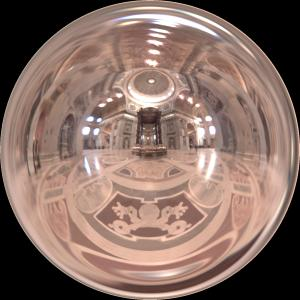
\includegraphics[width=0.4\textwidth]{Theory/example_probe}
\caption{Example of a light probe from St Peter's Basilica, Rome. Source\cite{website:PaulDebevec}}\label{fig:probe}
\end{figure}
\\ \\
When sampling a light probe it is therefore necessary to convert the 3 dimensional direction of the bent normal into a set of uv coordinates. We will now derive how. Since it is custom to have the center of the lightmap be the upwards direction we get that the base of the uv coordinates should be:
\[
(u,v) = (\frac{1}{2}, \frac{1}{2})
\]
the next part is to determine at what distance and in what direction from the center of the texture we should sample. Since we start from the middle of the texture the distance should go from 0 to 0.5. We can obtain this range by taking the arccos of the z value and divide by two pi:
\[
dist = \frac{arccos(D_z)}{2\pi}
\]
The x and y values tells us in what direction from the center we should go out to get to the right position. We therefore have to get the normalized xy vector:
\[
direction = \frac{1}{\sqrt{D_x^2 +D_y^2}} (D_x,D_y)
\]
At the end we can rearange to end up with the following:
\[
r = \frac{arcos(-D_z)}{2\pi\sqrt{D_x^2 + D_y^2}} 
\] \[
(u,v) = (\frac{1}{2}) + rD_x,\frac{1}{2}) + rD_y)
\]
Where D\textsubscript{x}, D\textsubscript{y} and D\textsubscript{z} is the lookup direction. Here it is assumed that the z-axis is upwards. One has also to take care of the event where Dx and Dy is close or equal to zero in which case the function should return (0.5 , 0.5). \newpage
\section{Disadvantages of Ambient Occlusion}
The main problem with Ambient Occlusion is from the fact that it reduces the problem of finding incident light, to using the calculated bent normal to do a texture lookup in an envirornment map. Since the bent normal is the average direction of incident light, it can in certain cases point in a direction that is actually occluded as illustrated by figure \ref{fig:bent_normal}.
\\
\begin{figure}[h!]
	\centering
	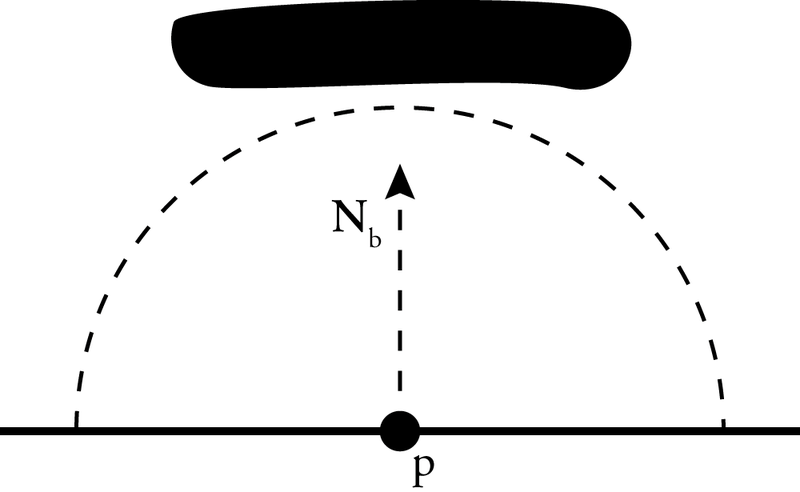
\includegraphics[width=0.5\textwidth]{Theory/bentNormalProblems}
\caption{The problem of using a bent normal Nb to find the irradiance at point P.}	\label{fig:bent_normal}
\end{figure}
\\ 
However since ambient occlusion is used to calculate the diffuse term the lookup into the envirornment map is usually blured which means this error is not so noticable.
\\ \\
The next section will cover our implementation of Ambient Occlusion.

\chapter{Implementation}
\section{Ambient Occlusion Shader}
To implement ambient occlussion in the ray tracing framework, it was necessary to create a new shader which can be found in  \texttt{Shaders\textbackslash{}DiffuseAmbientOccluded.cpp}. Later we implemented the functions that were needed to add support of HDR environment maps to our solution. This chapter will explain how different  methods needed to achieve it were implemented.  

\subsection{Rejection Sampling}
\label{sec:rejection_sampling}

First, we implemented a basic ambient occlusion shader which uses simple rejection sampling to generate rays to be traced from each point. The function called in \texttt{DiffuseAmbientOccluded::shade()} can be seen in 	\autoref{lst:rejection} while \autoref{lst:sampleHemi} shows the function \texttt{sampleHemisphere} responsible for the rejection sampling itself.

\lstinputlisting[caption = {Ambient occlusion shader with rejection sampling.}, label = {lst:rejection}]{Implementation/rejection.cpp}

The function in \autoref{lst:rejection} shoots a number of rays over the hemisphere as described in \cite{Gems17}. It calls the function from \autoref{lst:sampleHemi} to sample directions on the hemisphere.

\lstinputlisting[caption = {Rejection sampling.}, label = {lst:sampleHemi}]{Implementation/sampleHemi.cpp}

\subsection{Cosine Weighted Hemisphere}
\label{sec:cosine_weighted}
In order to improve performance and result of our solution we introduced the method of sampling ray directions from a cosine weighted hemisphere instead of the rejection sampling method used in the previous subsection. This provides a much more efficient way of generating rays distributed over a hemisphere and allows us to save computations. The relevant code is shown in \autoref{lst:sampleCosine}.

\lstinputlisting[caption = {Cosine weighted hemisphere sampling}, label = {lst:sampleCosine}]{Implementation/sampleCosine.cpp}

\section{Environment Sampling}
The next part of our project is to add sampling of light from the envirornment in form of HDR light probes. To do this we had to extend the framework to handle conversion from RGBE to floating point RGB as well as implement the projection of direction to texture coordinates. Then we could use them in our ambient occlusion solution.

\subsection{HDR Image Conversion}
The first part focuses on conversion of RGBE format used in HDR images to floating point RGB. This is done with the function from \autoref{lst:convert}.

\lstinputlisting[caption = {RGBE to RGBA conversion.}, label = {lst:convert}]{Implementation/convert.cpp}

\subsection{Spherical Texture Lookup}
Furthermore we needed to implement a function which returns coordinates in a spherical texture by converting direction from which the environment should be sampled to uv coordinates. This is done in \autoref{lst:project}.

\lstinputlisting[caption = {Conversion to texture coordinates}, label = {lst:project}]{Implementation/projectDirection.cpp}

In the end we could modify our shader code to include the contribution coming from the lookup in the spherical texture as shown in \autoref{lst:convert}.

\lstinputlisting[caption = {RGBE to RGBA conversion.}, label = {lst:convert}]{Implementation/environment.cpp}

\chapter{Results \& Discussion}
In the following chapter we will try to summarise the results we got from our ambient occlusion solution as well as compare the two implemented sampling methods and their efficiency with regard to the number of used samples.

\section{Comparison of ambient occlusion results}
This section contains comparison of results using rejection sampling (described in \autoref{sec:rejection_sampling}) to the use of cosine weighted hemisphere sampling (\autoref{sec:cosine_weighted}). The renders were run with 100, 200 and 300 sample rays and the results can be seen in \autoref{fig:AO_renders}.
\newline

The result clearly show that the cosine weighted hemisphere sampling performs much better than the simple rejection sampling. This may be accounted to higher efficiency of sampling the directions of rays.

\begin{figure}[h!]
	\centering
	\subfloat[100 samples, rejection sampling]{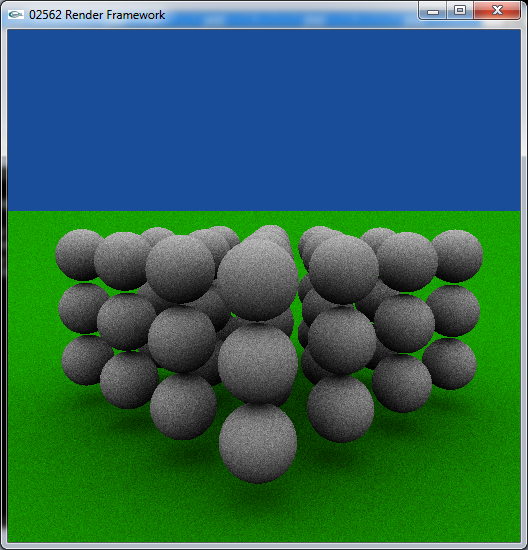
\includegraphics[width=.4\textwidth]{Results/rejection100.png}}
    	\subfloat[100 samples, cosine weighted sampling]{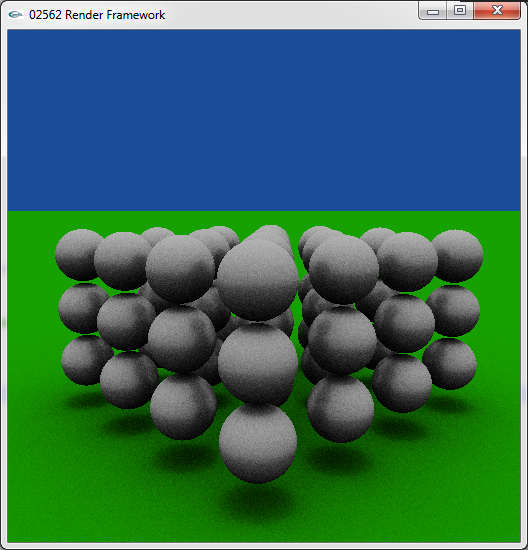
\includegraphics[width=.4\textwidth]{Results/cosine100.png}}\\
    	\subfloat[200 samples, rejection sampling]{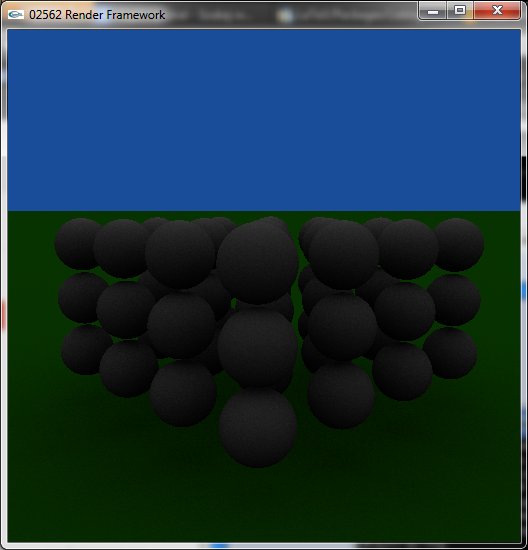
\includegraphics[width=.4\textwidth]{Results/rejection200.png}}
    	\subfloat[200 samples, cosine weighted sampling]{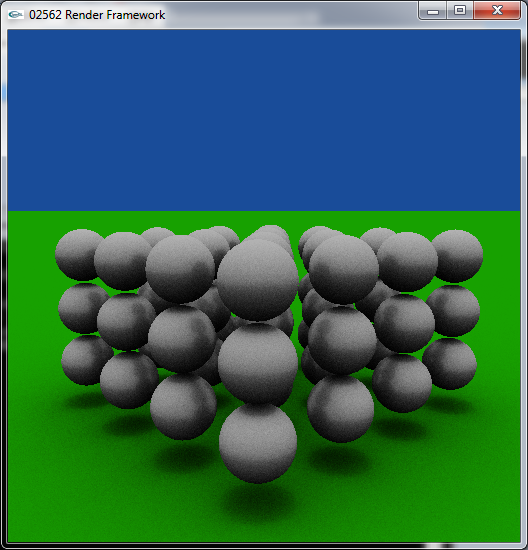
\includegraphics[width=.4\textwidth]{Results/cosine200.png}}\\
	\subfloat[300 samples, rejection sampling]{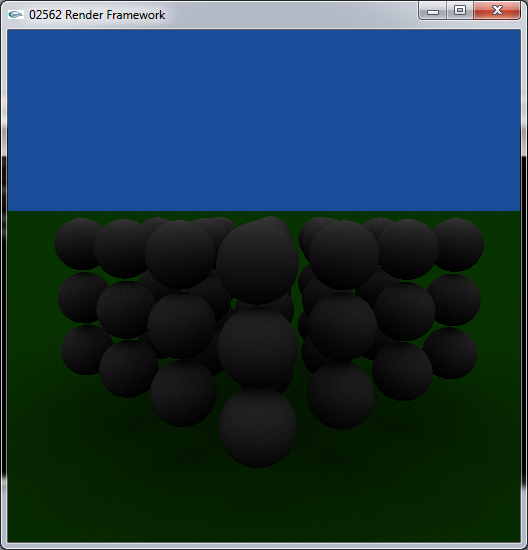
\includegraphics[width=.4\textwidth]{Results/rejection300.png}}
    	\subfloat[300 samples, cosine weighted sampling]{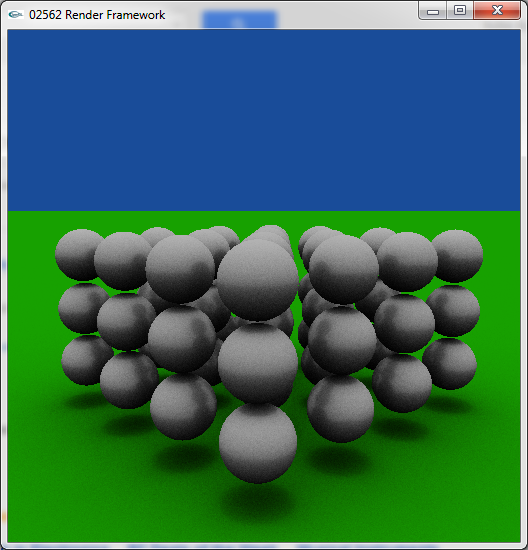
\includegraphics[width=.4\textwidth]{Results/cosine300.png}}\\
	\caption{Comparison of sampling methods if different number of samples}
	\label{fig:AO_renders}
\end{figure}

\begin{figure}[h!]
	\centering
	\subfloat[100 samples, rejection sampling]{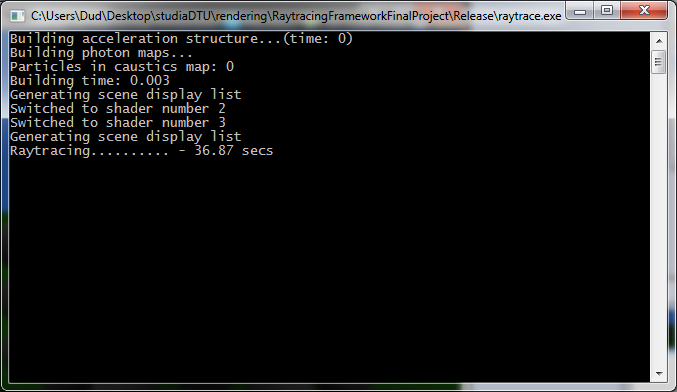
\includegraphics[width=.4\textwidth]{Results/rejection100_log.png}}
    	\subfloat[100 samples, cosine weighted sampling]{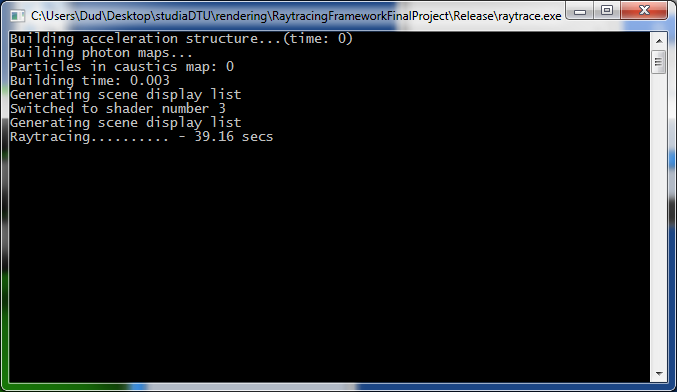
\includegraphics[width=.4\textwidth]{Results/cosine100_log.png}}\\
    	\subfloat[200 samples, rejection sampling]{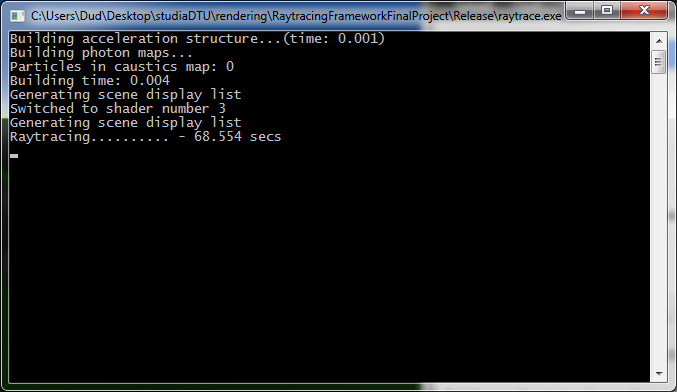
\includegraphics[width=.4\textwidth]{Results/rejection200_log.png}}
    	\subfloat[200 samples, cosine weighted sampling]{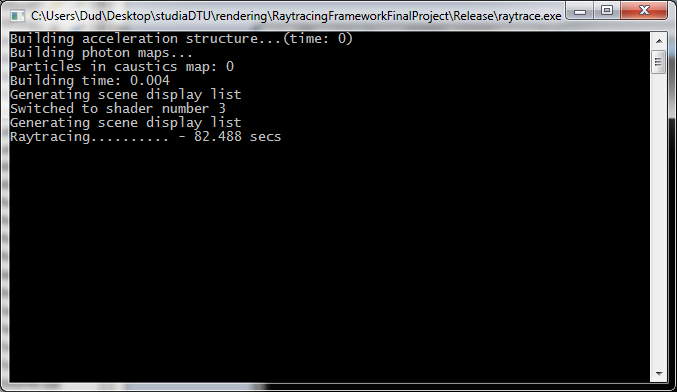
\includegraphics[width=.4\textwidth]{Results/cosine200_log.png}}\\
	\subfloat[300 samples, rejection sampling]{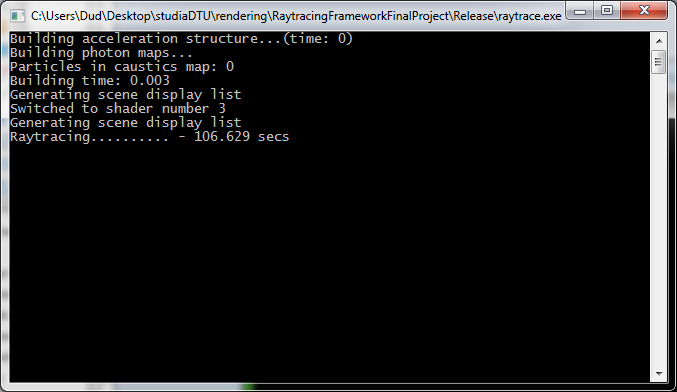
\includegraphics[width=.4\textwidth]{Results/rejection300_log.png}}
    	\subfloat[300 samples, cosine weighted sampling]{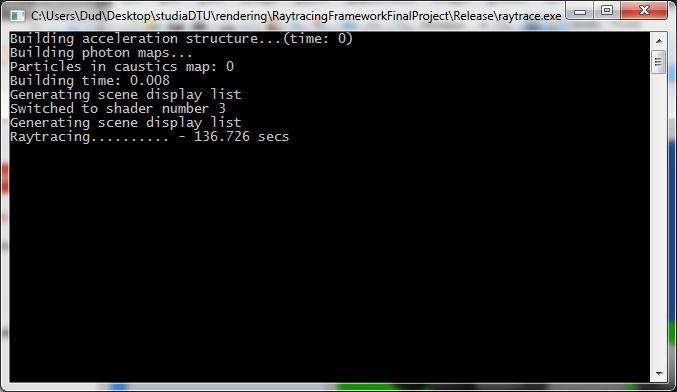
\includegraphics[width=.4\textwidth]{Results/cosine300_log.png}}\\
	\caption{Render logs for the renders in \autoref{fig:AO_renders}.}
	\label{fig:AO_logs}
\end{figure}
\section{HDR environment map}
The final feature that we included in our ambient occlusion solution is environment mapping from HDR textures (as seen in \autoref{sec:environment_maps}). The renders in \autoref{fig:env_renders} use the cosine weighted hemisphere sampling method implemented in the previous chapter. 
\begin{figure}[h!]
	\centering
	\subfloat[Render with Grace Cathedral texture.]{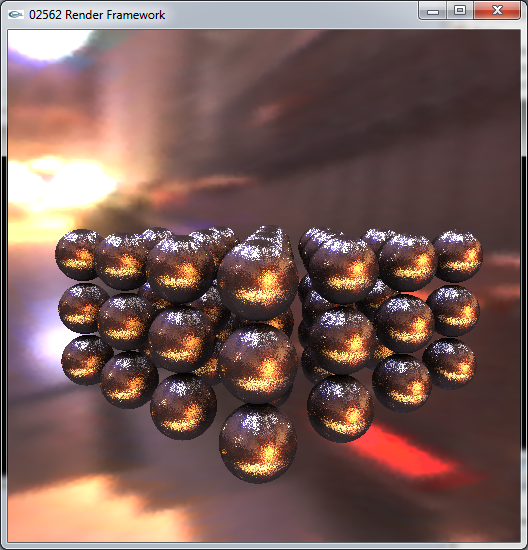
\includegraphics[width=.4\textwidth]{Results/hdr.png}}
    	\subfloat[Render log.]{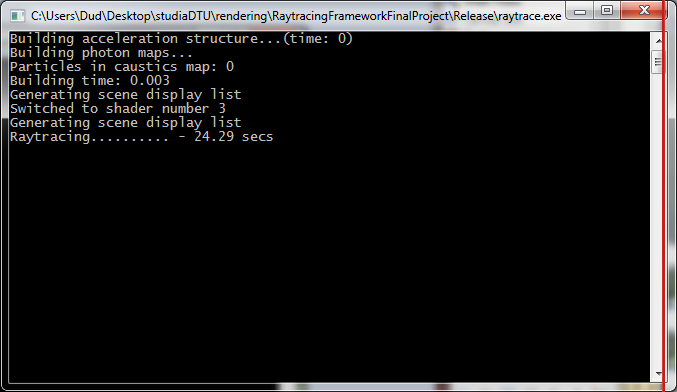
\includegraphics[width=.4\textwidth]{Results/hdr_log.png}}\\
    	\subfloat[Render with Campus at Sunset texture.]{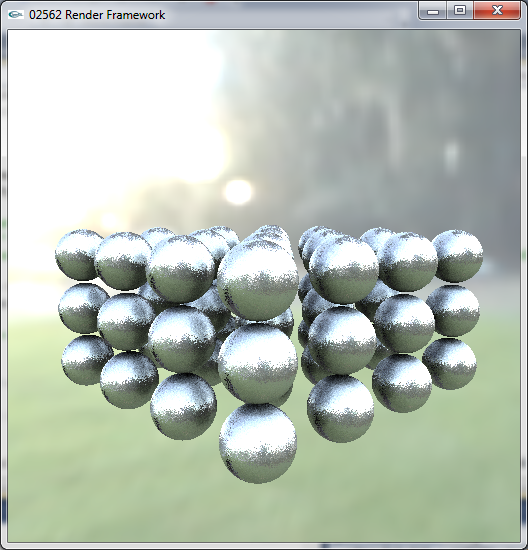
\includegraphics[width=.4\textwidth]{Results/hdr1.png}}
    	\subfloat[Render log.]{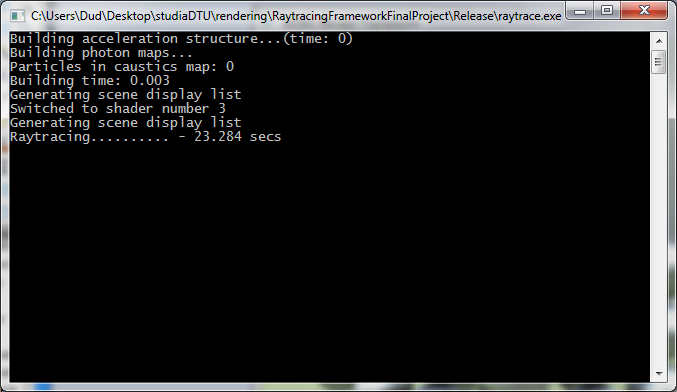
\includegraphics[width=.4\textwidth]{Results/hdr1_log.png}}\\
	\caption{Environment mapping results.}
	\label{fig:env_renders}
\end{figure}
The HDR images used in renders in \autoref{fig:env_renders} come from \cite{website:PaulDebevec}

\chapter{Conclusion}
We have demonstrated two different ways of performing the sampling for ambient occlusion that produced two different visual results. From the litterature it seems that both methods are acceptable so it is a matter of what visual style that fits the desired result the best. That the two different methods produce two overall different levels of brightness. A likely candidate is the lack of a modification with the probability density function in the rejection sampling method but it does not seem to be something that other papers take into consideration \cite{Gems17}. The lookup into the light probe image and conversion from the RGBE format to floating point RGB seems to work in a satisfactory way.
\\ \\
The two most obvious improvements to our method would be to change the weight of each occluded ray based on how far away the hit on the occluder are. Another improvement would be to implemnt a blurred lookup into the envirornment map.

\bibliographystyle{siam}
%\bibliography{Bibliography/HCI}
\bibliography{Bibliography/Alexanders,Bibliography/Jacubs}
\end{document}